% !TEX encoding = UTF-8 Unicode

\documentclass[11pt, a4paper]{article}

\usepackage[utf8]{inputenc}
\usepackage[pdftex]{graphicx}
\usepackage{amsmath}

\addtolength{\textwidth}{1.75in}
\addtolength{\oddsidemargin}{-.875in}
\addtolength{\evensidemargin}{-.875in}
\addtolength{\topmargin}{-70pt}
\addtolength{\textheight}{70pt}
 
\begin{document}
%\begin{center}
{\noindent \huge \bf Active Learning Model Results}\\


\section*{The Model}
The model we use is a hierarchical model with three levels: the \emph{theory} level, the \emph{hypotheses} level, and the \emph{data} level, and is depicted in figure~\ref{fig:model}. At the \emph{theory} level, there is a single variable $t$ indexing the different theories. At the \emph{hypotheses} level, there is one variable $h_i$ indexing hypotheses for each machine $i\in\{1,2,3\}$. Finally, \emph{data} $\mathbf d_i$ is split according to which machine it corresponds to, and the bold notation denotes many single datapoints or \emph{actions} (placing a toy against a machine to see whether it lights up or not). Finally, toys and machines have two properties, color and shape, of arbitrary dimensions $n_c$ and $n_s$. 
\begin{figure}[ht]
\begin{center}
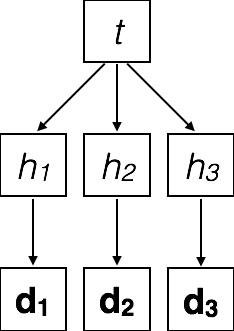
\includegraphics[width=0.25\textwidth]{Model.png}
\end{center}
\caption{Model structure}
\label{fig:model}
\end{figure}

\subsection*{The \emph{theory} level}
We consider the following 12 theories:\\
\begin{tabular}{|c|c|}
\hline
t & theory \\
\hline
0 & No block works\\
1 & Any block works\\
2 & Matching color\\
3 & Matching shape\\
4 & Match color \& shape\\
5 & Match color or shape\\
6 & Any specific color\\
7 & Any specific shape\\
8 & Specific color and shape\\
9 & Nonmatching color\\
10 & Nonmatching shape\\
11 & Independent \\
\hline
\end{tabular}\\
We take a flat prior for the theories, $p(t)=1/12$. 

\subsection*{The \emph{hypotheses} level}
For each machine $i$, we consider the following hypotheses, sorted into different kinds:\\
\begin{tabular}{|c|c|c|c|}
\hline
kind  & amount & $h_i$ & hypotheses \\
\hline
0 & 1& 0 & No block works\\
1 & 1 & 1 & Any block works\\
2 & $n_c$ & [2, 2+$n_c$) & Specific color\\
3 & $n_s$ & [2+$n_c$, 2+$n_c$+$n_s$) & Specific shape\\
4 & $n_c$$n_s$ & [2+$n_c$+$n_s$, 2+$n_c$+$n_s$+$n_c$$n_s$) & Specific color \& shape\\
5 & $n_c$$n_s$ & [2+$n_c$+$n_s$+$n_c$$n_s$, 2+$n_c$+$n_s$+2$n_c$$n_s$) & Specific color or specific shape\\
6 & $n_c\choose2$ & [2+$n_c$+$n_s$+2$n_c$$n_s$, 2+$n_c$+$n_s$+2$n_c$$n_s$+$n_c\choose2$) & Two specific colors\\
7 & $n_s\choose2$&  [2+$n_c$+$n_s$+2$n_c$$n_s$+$n_c\choose2$, 2+$n_c$+$n_s$+2$n_c$$n_s$+$n_c\choose2$+$n_s\choose2$) &Two specific shapes\\
\hline
\end{tabular}
There are a total of $n_h=2+n_c+n_s+2 n_c n_s+ {n_c \choose 2 }+ {n_s \choose 2}$ hypotheses per machine. 


\subsection*{The theory-hypothesis likelihood}
Theories are linked to hypotheses for each machine through the following likelihood, $p(h_i|t)$ (omitting zeros for clarity):\\
\begin{tabular}{|c|c|c|c|c|c|c|c|c|}
\hline
$t/h_i$ kind & 0 & 1 & 2 & 3 & 4 & 5 & 6 & 7 \\
\hline
0 & 1 & & & & & & & \\
1 & & 1 & & & & & &\\
2 & & & 1 & & & & &\\
3 & & & & 1 & & & &\\
4 & & & & & 1 & & &\\
5 & & & & & & 1 & &\\
6 & & & 1/$n_c$ & & & & &\\
7 & & & & 1/$n_s$ & & & &\\
8 & & & & & 1/$n_c$$n_s$ & & &\\
9 & & & $\frac{1}{n_c-1}$ & & & & $\frac{1}{{n_c\choose 2} -(n_c-1)} $ &\\
10 & & & & $\frac{1}{n_s-1}$ & & & &$\frac{1}{{n_s\choose 2} -(n_s-1)} $ \\
11 & $1/n_h$ & $1/n_h$ & $1/n_h$ & $1/n_h$ & $1/n_h$ & $1/n_h$ & $1/n_h$ & $1/n_h$ \\
\hline
\end{tabular}

\subsection*{The \emph{data} level and the data-hypothesis likelihood}
Single datapoints are (\emph{toy},\emph{machine}) pairs, together with a \emph{result} $\in\{ \textrm{True, False} \}$, indicating whether the machine lit up or not. Data are thus split according to their corresponding machine, and each machine's data are independent from the rests', conditioned on the corresponding hypothesis. The likelihood then factorizes as follows:
\begin{equation}
p(\textbf d_1, \textbf d_2, \textbf d_3| h_1, h_2, h_3)=p(\textbf d_1| h_1)p(\textbf d_2| h_2)p(\textbf d_3| h_3).
\end{equation}
Each machine's data $\textbf d_i$ in turn a collection of datapoints $d_i$ corresponding to that machine. These different datapoints are again conditionally independent given the hypothesis, such that we only need look at the likelihood for a single datapoint $d_i$:
\begin{equation}
p(d_i| h_i)= \begin{cases} 
				1  & \textrm{if $d_i$ is compatible with  $h_i$} \\
                   	\epsilon &  \textrm{if it is not}, \\
                   \end{cases}
\end{equation}
where $\epsilon$ is a free noise parameter. Compatibility here means that the toy in $d_i$ satisfies the criteria specified by $h_i$ for the machine to activate, if the state of the machine in $d_i$ is active, or that the toy fails to satisfy the criteria in $h_i$, and the state of the machine is inactive. As an example, a machine being activated with a blue toy is compatible with the \emph{blue toys} hypothesis, as is a machine not being activated by a red toy. 

\subsection*{Full model}
With these ingredients, the full joint distribution factors as:
\begin{equation}
p(\textbf d_1,\textbf d_2,\textbf d_3,h_1,h_2,h_3,t)=\left[\prod_{i=1}^3 p(\textbf d_i|h_i) p(h_i|t) \right]p(t)
\end{equation}

\subsection*{Active learning}
We implement three different active learner models, all based on the model above, but each seeking to maximize information gain at a different level. Although the three learners vary in which distribution they focus on, the general expression for the expected information gain is the same:
\begin{equation}
\textrm{EIG}(a)=-\sum_{d^{new}} \bigg( H[p(\dots|d^{new},{\textbf d^{old}})]-H[p(\dots|{\textbf d^{old}})] \bigg) p(d^{new}| a, {\textbf d^{old}}),
\end{equation}
where the sum is over all possible data $d^{new}$ consistent with action $a$ (that is, the machine lighting or not), and $\textbf d^{old}$ is all accumulated data prior to the action choice. The dots in the probability distributions stand for the arguments each learner is concerned with: $t$ for the \emph{theory} learner, $h_1, h_2, h_3$ for the \emph{hypotheses} learner, and $t, h_1, h_2, h_3$ for the \emph{joint} theory-hypotheses learner. Finally, we note that the second term in the difference does not depend on the action choice, yielding a constant term that we can omit, leaving the learners with the problem of minimizing the expected final entropy:
\begin{equation}
\textrm{EFE}(a)=\sum_{d^{new}} H[p(\dots|d^{new},{\textbf d^{old}})] p(d^{new}| a, {\textbf d^{old}}).
\label{eig}
\end{equation}
Working with this quantity is equivalent to using the EIG when taking differences, since the constants cancel out.

The $p(d^{new}| a, {\textbf d^{old}})$ in the equations above is the probability of finding each piece of data $d^{new}$ given an action $a$ and prior experience ${\textbf d^{old}}$, and is the same for all models:
\begin{equation}
\begin{split}
%p(d^{new}| a, {\textbf d^{old}})=&\sum_{h_i} p(d_i^{new}|a, h_i, {\textbf d^{old}}) p(h_i|a, {\textbf d^{old}})=\\
%&\sum_{h_i,t} p(d_i^{new}|a, h_i) p(h_i| {\textbf d^{old}}, t) p(t|{\textbf d^{old}})=\\
%&\sum_{h_i,t} p(d_i^{new}|a, h_i) p(h_i | t) \frac{p({\textbf d_i^{old}} | h_i)}{p({\textbf d_i^{old}} | t)} p(t|{\textbf d^{old}}),
p(d^{new}| a, {\textbf d^{old}})=&\sum_{h_i} p(d_i^{new}|a, h_i, {\textbf d^{old}}) p(h_i|a, {\textbf d^{old}})=\\
&\sum_{h_i} p(d_i^{new}|a, h_i) \sum_t p(h_i| {\textbf d^{old}}, t) p(t|{\textbf d^{old}})=\\
&\sum_{h_i,t} p(d_i^{new}|a, h_i) p(h_i| {\textbf d^{old}_i}, t) p(t|{\textbf d^{old}})=\\
&\sum_{h_i,t} p(d_i^{new}|a, h_i) \frac{p({\textbf d_i^{old}} | h_i) p(h_i | t)}{p({\textbf d_i^{old}} | t)} p(t|{\textbf d^{old}}),
%{\textbf d^{old}}, t) p(t|{\textbf d^{old}})
\end{split}
\label{paction}
\end{equation}
where some index magic took place. First, we converted $d^{new}$ to $d_i^{new}$, which only amounts to saying that a single datapoint can only correspond to an individual machine, labeled $i$, which is the one whose hypotheses we sum over on the RHS. Second, from the second to the third line, we see ${\textbf d^{old}}$ reduced to ${\textbf d_i^{old}}$. This is because of hypothesis $h_i$ being independent of data in other machines given the theory. Finally, we used Bayes' theorem and the fact that data are independent of the theory given the hypothesis in the corresponding machine to go from the third to the last line. 
%\begin{equation}
%\begin{split}
%p(h_i| {\textbf d}, t)=p(h_i| {\textbf d_1}, {\textbf d_2}, {\textbf d_3}, t)=p(h_i | {\textbf d_i}, t)=\frac{p(h_i , {\textbf d_i} |t )}{p ({\textbf d_i} | t)} =
%\frac{p( {\textbf d_i}|h_i,t)p(h_i|t)}{p( {\textbf d_i} | t)}=\frac{p(h_i|t)p( {\textbf d_i}|h_i)}{p( {\textbf d_i} | t)},
%\end{split}
%\end{equation}
%where we suppressed the superscripts for clarity. 
This leaves us with two more things to compute in~\eqref{paction}: the theory posterior $p(t|{\textbf d})$, and $p({\textbf d_i} | t)$. This last probability is given by:
\begin{equation}
p({\textbf d_i} | t) = \sum_{h_i} p({\textbf d_i} | h_i) p(h_i | t),
\end{equation}
whereas the expression for the theory posterior is shown below.

\subsubsection*{Theory learner}
The theory learner seeks to minimize the EFE given in equation~\eqref{eig} for the theory posterior:
\begin{equation}
p(t | {\textbf d_1}, {\textbf d_2}, {\textbf d_3}) \propto p({\textbf d_1}, {\textbf d_2}, {\textbf d_3}|t) p(t)
\end{equation}
with
\begin{equation}
p( {\textbf d_1}, {\textbf d_2}, {\textbf d_3} |t) = \prod_i \sum_{h_i} p({\textbf d_i} | h_i) p(h_i | t).
\end{equation}

\subsubsection*{Hypotheses learner}
The hypotheses learner seeks to minimize the EFE given in equation~\eqref{eig} for the hypotheses posterior:
\begin{equation}
\begin{split}
p(h_1, h_2, h_3 | {\textbf d_1}, {\textbf d_2}, {\textbf d_3}) \propto p({\textbf d_1}, {\textbf d_2}, {\textbf d_3} | h_1, h_2, h_3)=
\sum_t \Big( \prod_i p({\textbf d_i} | h_i) p(h_i | t) \Big) p(t).
\end{split}
\end{equation}

\subsubsection*{Joint learner}
The joint theory/hypotheses learner seeks to minimize the EFE given in equation~\eqref{eig} for the joint posterior:
\begin{equation}
\begin{split}
p(h_1, h_2, h_3, t | {\textbf d_1}, {\textbf d_2}, {\textbf d_3}) \propto \Big( \prod_i p({\textbf d_i} | h_i) p(h_i | t) \Big) p(t).
\end{split}
\end{equation}




%%%%%%%%%%%%%%%%%%%%%%%%%%%%

\section*{Results}
Summary of results so far. For all learners, we will evaluate the difference in EIG between the kids and the optimal model learner (red in the histograms, y axes in scatter plots), as well as the difference between a random choice model and the optimal learner (blue and x axes). We study these differences for each action in the playing sequence, feeding the model learners the actual kids' gameplay up to the given choice. All random results are averaged over 20 realizations, and we set a value of $\epsilon=0.001$.

\subsection*{Theory learner}
The results for this learner are presented in figures~\ref{fig:th} and \ref{fig:ts}.% and table~\ref{tab:t}.

\begin{figure}[h!]
\begin{center}
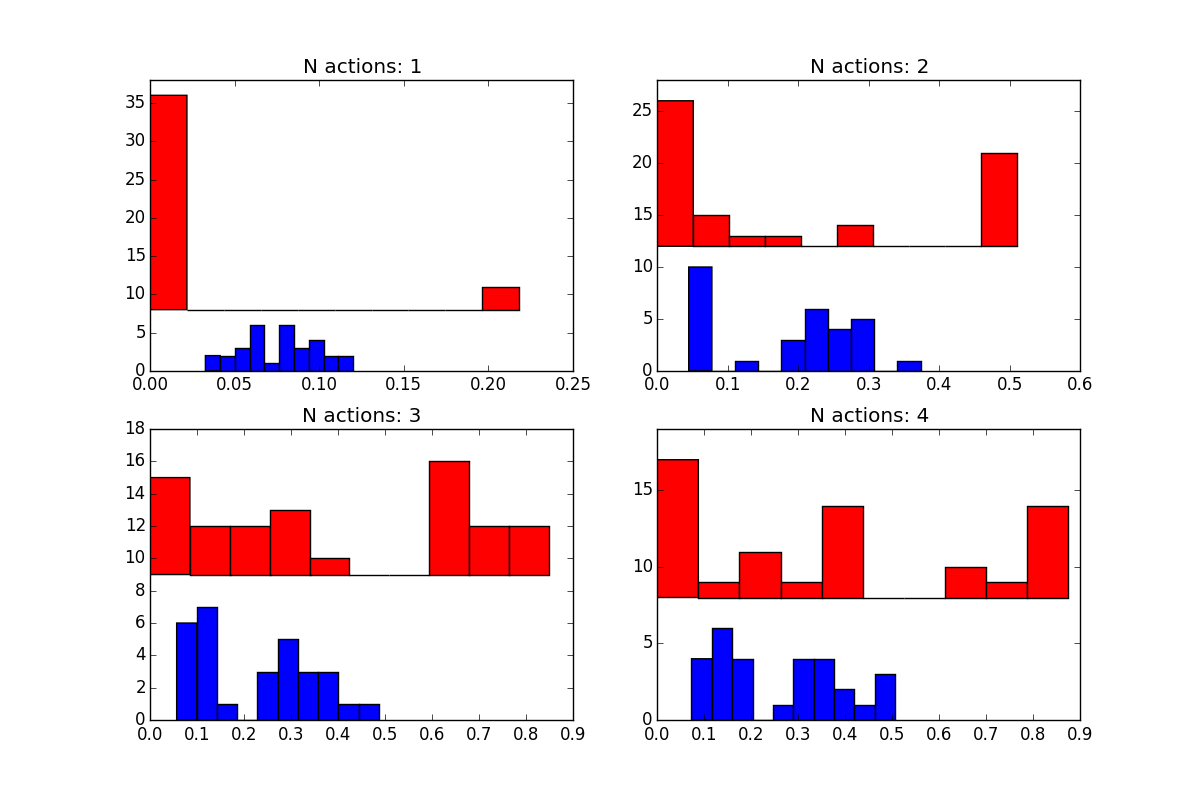
\includegraphics[width=0.75\textwidth]{../Plots/IG_theory_hist.png}
\end{center}
%\vspace{-1cm}
\caption{Theory model EIG histograms. Kids - optimal (red) and random - optimal (blue)}
\label{fig:th}
\end{figure}

\begin{figure}[h!]
\begin{center}
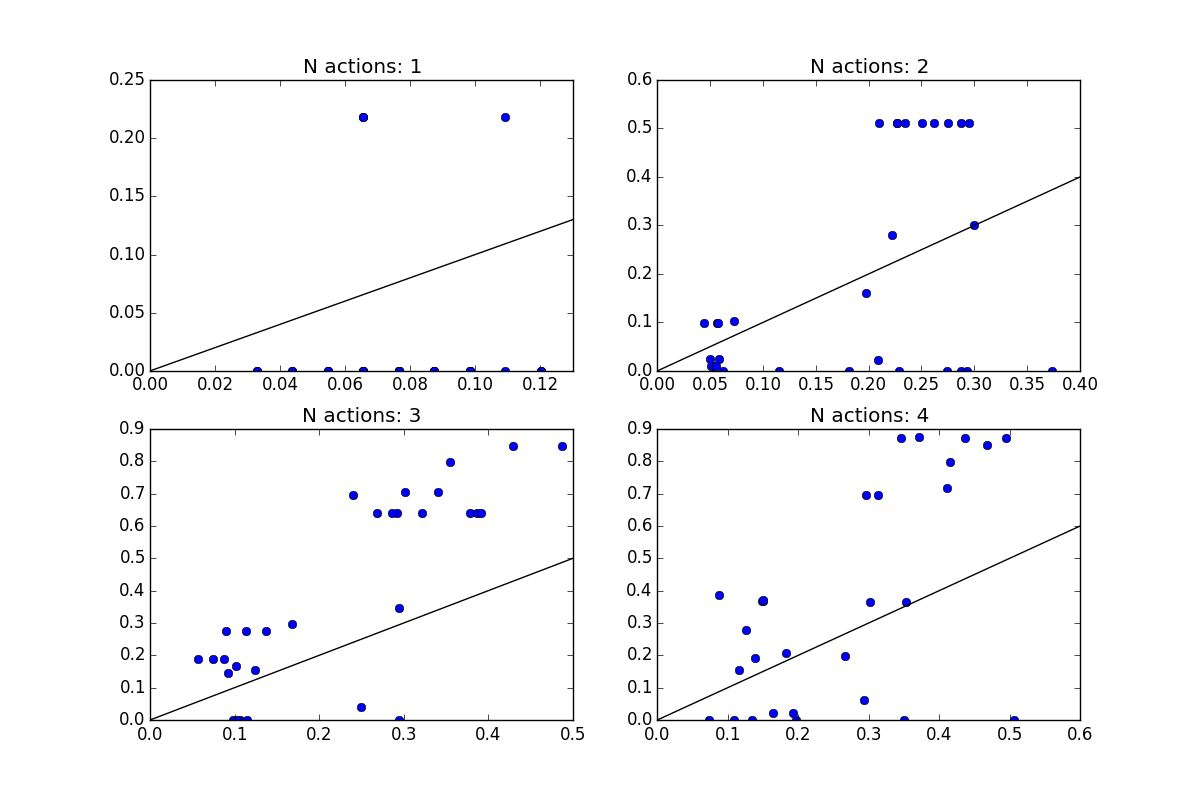
\includegraphics[width=0.75\textwidth]{../Plots/IG_theory_scat.png}
\end{center}
%\vspace{-1cm}
\caption{Theory model EIG scatterplots. Kids - optimal (y axes) vs random - optimal (x axes). Kids below the identity line perform better than random.}
\label{fig:ts}
\end{figure}


\clearpage
\subsection*{Hypotheses learner}
The results for this learner are shown in figures~\ref{fig:hh} and \ref{fig:hs}.% and table~\ref{tab:h}.
\begin{figure}[h!]
\begin{center}
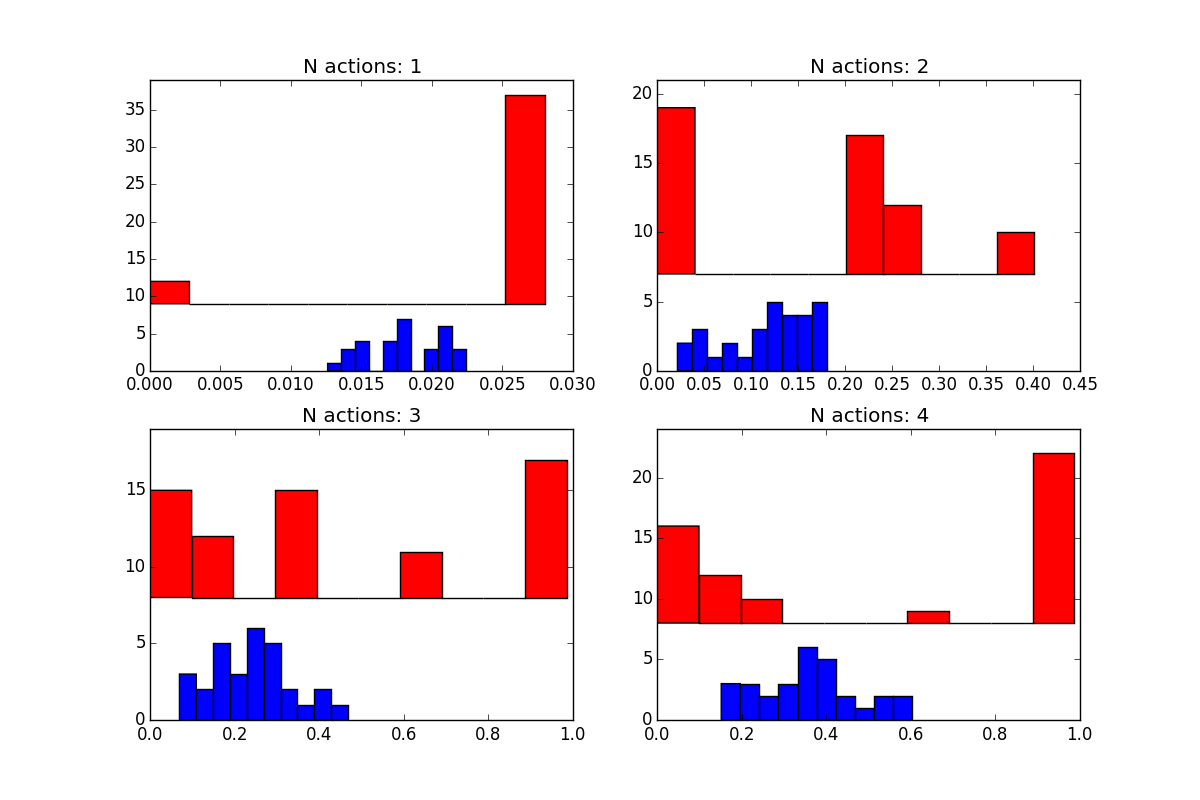
\includegraphics[width=0.75\textwidth]{../Plots/IG_hyp_hist.png}
%\vspace{-1cm}
\caption{Theory model EIG histograms. Kids - optimal (red) and random - optimal (blue)}
\label{fig:hh}
\end{center}
\end{figure}
\begin{figure}[h!]
\begin{center}
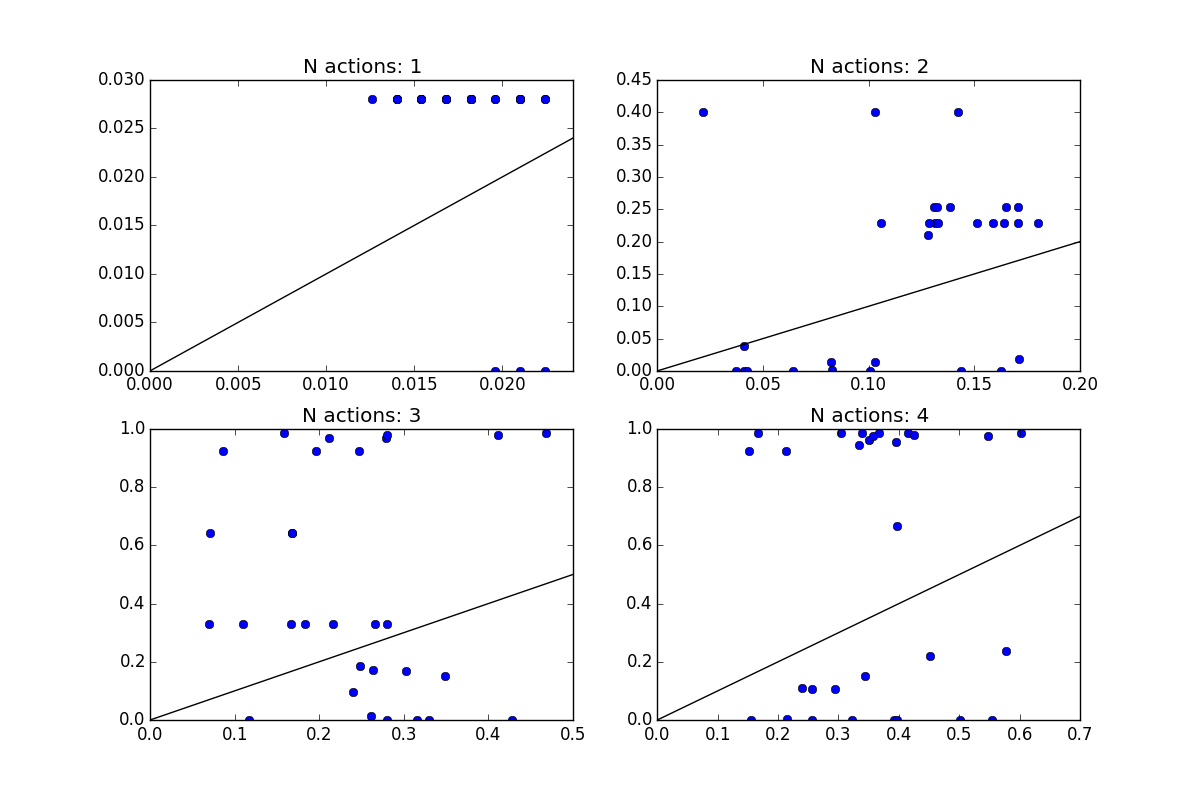
\includegraphics[width=0.75\textwidth]{../Plots/IG_hyp_scat.png}
%\vspace{-1cm}
\caption{Hypotheses model EIG scatterplots. Kids - optimal (y axes) vs random - optimal (x axes). Kids below the identity line perform better than random.}
\label{fig:hs}
\end{center}
\end{figure}






\clearpage
\subsection*{Joint learner}
The results for this learner are presented in figures~\ref{fig:jh} and \ref{fig:js}.% and table~\ref{tab:j}.

\begin{figure}[h!]
\begin{center}
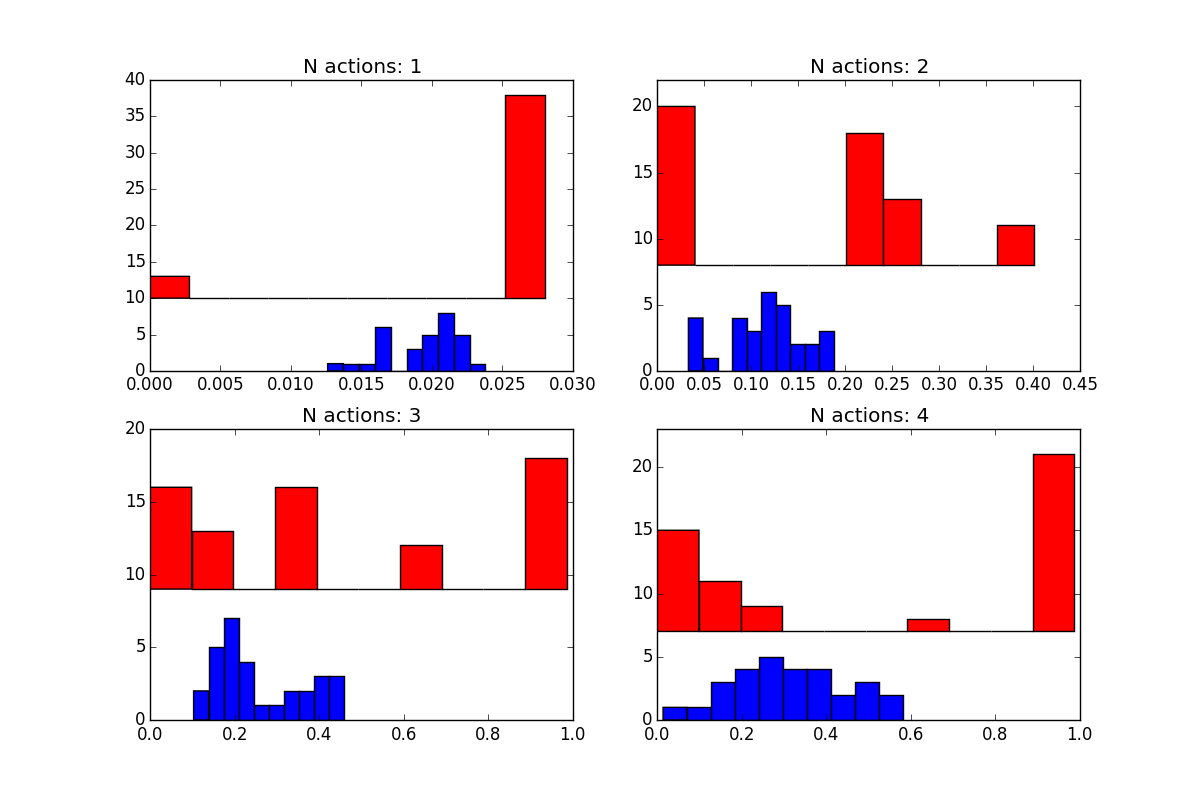
\includegraphics[width=0.75\textwidth]{../Plots/IG_joint_hist.png}
\end{center}
%\vspace{-1cm}
\caption{Joint model EIG histograms. Kids - optimal (red) and random - optimal (blue)}
\label{fig:jh}
\end{figure}

\begin{figure}[h!]
\begin{center}
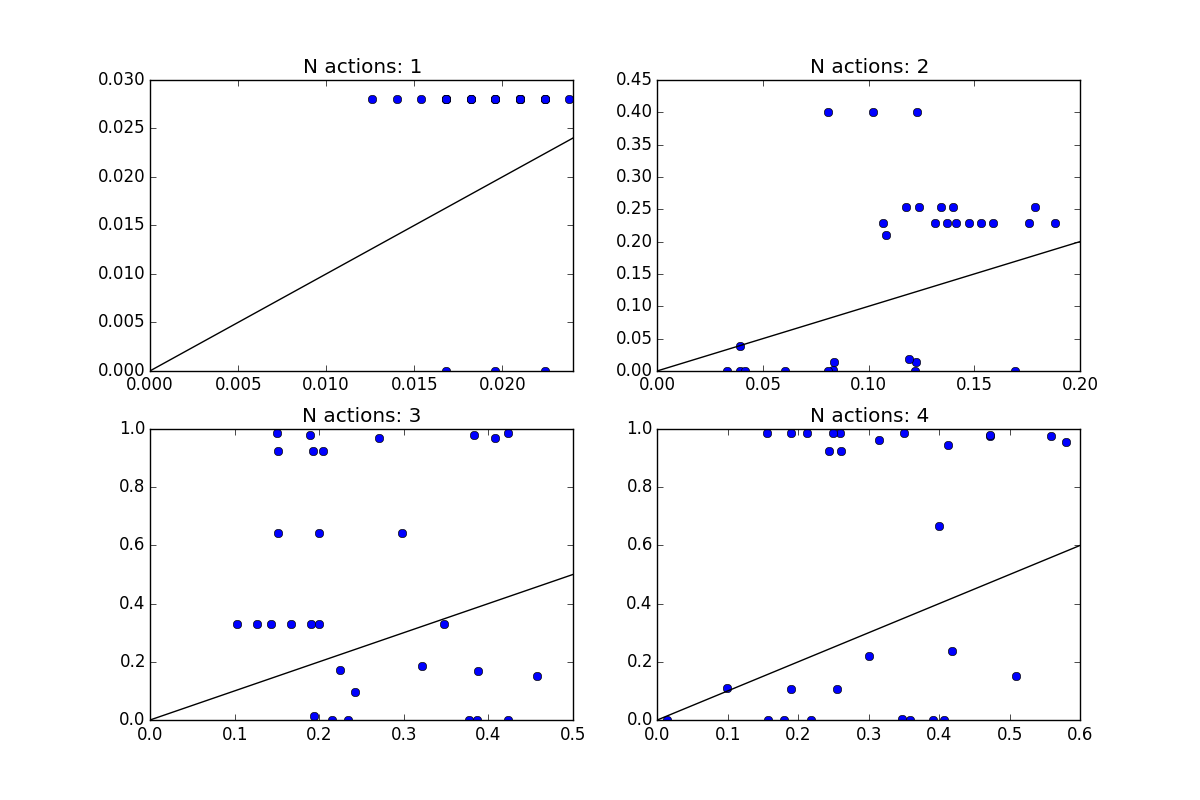
\includegraphics[width=0.75\textwidth]{../Plots/IG_joint_scat.png}
\end{center}
%\vspace{-1cm}
\caption{Joint model EIG scatterplots. Kids - optimal (y axes) vs random - optimal (x axes). Kids below the identity line perform better than random.}
\label{fig:js}
\end{figure}




\clearpage
\subsection*{All learners}
A summary of the results through paired $t$-test for the different actions and different models is shown in the following table. Positive $t$ means kids better than random. 
%\begin{table}[h!]
\begin{center}
\begin{tabular}{|c||c|c||c|c||c|c|}
\hline
%\cline{2-5}
model & \multicolumn{2}{|c||}{theory} & \multicolumn{2}{|c||}{hypotheses} & \multicolumn{2}{|c|}{joint} \\
\hline
\# actions & $t$ & $p$ & $t$ & $p$ & $t$ & $p$\\
\hline
1 & 4.473 & 0.000 & -4.089 & 0.000 & -3.718 & 0.001\\
2 & -0.301 & 0.766 & -1.845 & 0.075 & -2.064 & 0.048\\
3 & -4.292 & 0.000 & -2.939 & 0.006 & -2.635 & 0.013\\
4 & -2.060 & 0.049 & -1.925 & 0.064 & -2.602 & 0.015\\
\hline
\end{tabular}
\end{center}


\subsection*{Varying $\epsilon$}
We varied the parameter $\epsilon$ for the theory model to analyze how the predictions changed. The results are shown in figure~\ref{fig:varye}. In the figure the $t$ statistics (green) and $p$ values (purple) for the test in the previous section are shown as a functin of $\epsilon$, for different action numbers. $t$ values below 0 (black dotted line) indicate kids doing better than chance, with significance assessed by the corresponding $p$ value. Kids are better than chance in their first action choice for all values of $\epsilon$. For other action numbers, they are always worse than chance or similar to it apart from the second action, in which they are better for $\epsilon=0.25$. 
\begin{figure}[h!]
\begin{center}
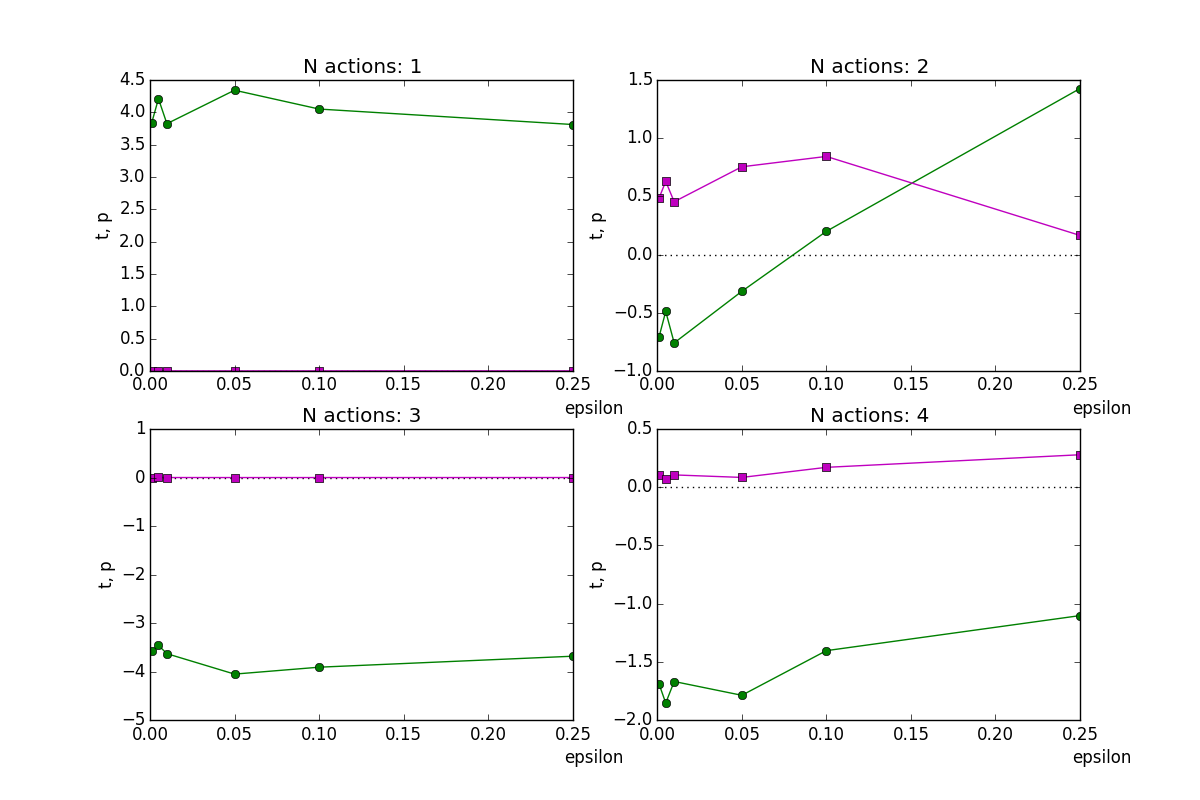
\includegraphics[width=0.75\textwidth]{../Plots/vary_ep_theory.png}
\end{center}
%\vspace{-1cm}
\caption{Theory model $\epsilon$ dependence. $t$ statistic (green) and $p$ value (purple) for tests in previous section as a function of $\epsilon$, for the different action numbers (panels).}
\label{fig:varye}
\end{figure}

\subsection*{Scrutinizing (second) action choices}
We look at kids' choice of second action, depending on their first choice. We categorize the first choice as successful matches (a toy/machine match with the correct property according to the specific condition, $a_1=+$), unsuccessful matches (a toy/machine match with the opposite property, $a_1=-$) and nonmatches (toy and machine different in color and shape, machine always inactive, $a_1={\textrm N}$). The second choice can be split according to 6 categories as follows (I use numbers for notation). Same property as first action, different toy and machine: $a_2=0$. Same machine as $a_1$, but matching the opposite property, $a_2=1$. Same toy as $a_1$, opposite property $a_2=2$. Same machine as $a_1$, no match between toy and machine, $a_2=3$. Same toy as $a_1$, no match between toy and machine, $a_2=4$. Different toy and machine than $a_1$, nonmatching either, $a_2=5$. Note that categories $a_2=3$ and $a_2=4$ are unsatisfiable for $a_1=n$, and that the number of actions that feeds each category varies between 1 and 2, what must be taken into account when considering random choices. 

In the following table, we sort kids' second choice of action as a function of their first one. Entries are number of kids in each condition. 30 kids are considered in total, dropping one that only made one action: 
\begin{center}
\begin{tabular}{|c||c|c|c|}
\hline
$a_2 / a_1$ & + & - & N\\
\hline\hline
0 & 10 & 3 & 1 \\ 
1 & 5 & 3 & 2 \\ 
2 & 0 & 1 & 0 \\ 
3 & 1 & 2 & 0 \\ 
4 & 1 & 0 & 0 \\ 
5 & 0 & 1 & 0 \\ 
\hline
\end{tabular}
\end{center}
The theory model gives the following expected final entropies for these actions:
\begin{center}
\begin{tabular}{|c||c|c|c|}
\hline
$a_2 / a_1$ & + & - & N\\
\hline\hline
0 & 1.843 & 2.084 & 2.731 \\ 
1 & {\bf 1.331} & 1.995 & {\bf 2.570} \\ 
2 & 1.354 & {\bf 1.986} & 2.731 \\ 
3 & 1.612 & 2.011 & -- \\ 
4 & 1.632 & 2.089 & -- \\ 
5 & 1.632 & 2.089 & 2.906 \\ 
\hline
\end{tabular}
\end{center}
where we marked in bold the correct second action given the first. The model essentially tells us to try the property opposite to that already tried, whether we were successful or not on the first try. Only 8 kids out of 30 get the perfect choice, and 12 out of 30 if we include marginally suboptimal choices. The remaining kids make bad choices. In particular, the 10 kids with $a_1=+$ and $a_2=0$ choose to repeat their successful property match, but either changing the toy or the machine, which is the worst possible action to take according to the model.

Setting $\epsilon=0.25$, the best fitting value for the second action choice, we get for the entropies:
\begin{center}
\begin{tabular}{|c||c|c|c|}
\hline
$a_2 / a_1$ & + & - & N\\
\hline\hline
0 & 2.547 & 2.563 & 3.052 \\ 
1 & {\bf 2.506} & 2.543 & {\bf 3.031} \\ 
2 & 2.508 & {\bf 2.541} & 3.052 \\ 
3 & 2.572 & 2.573 & -- \\ 
4 & 2.571 & 2.581 & --\\ 
5 & 2.571 & 2.581 & 3.091 \\ 
\hline
\end{tabular}
\end{center}
We see that the model still suggests the same actions, which speaks about its robustness. Other action combinations vary in value, which explains how children can in this setting be better than chance. 

The hypotheses model predicts, for the extreme values of $\epsilon$ considered:
\begin{center}
\begin{tabular}{|c||c|c|c||c|c|c|}
\hline
 & \multicolumn{3}{|c||}{$\epsilon=0.001$} & \multicolumn{3}{|c|}{$\epsilon=0.25$}\\
 \hline
$a_2 / a_1$ & + & - & N  &+ & - & N\\
\hline\hline
0 & 4.332 & 5.792 & 5.186 & 6.023 & 6.571 & 6.509 \\ 
1 & 4.355 & {\bf 5.391} & {\bf 5.147} & 6.057 & {\bf 6.496} & {\bf 6.501} \\ 
2 & 4.313 & {\bf 5.391} & 5.186 & 6.052 & 6.497 & 6.509 \\ 
3 & {\bf 4.102} & 5.405 & -- & {\bf 6.013} & 6.499 & -- \\ 
4 & 4.120 & 5.392 & -- & 6.017 & {\bf 6.496} & -- \\ 
5 & 4.120 & 5.392 & 5.225 & 6.017 & {\bf 6.496} & {\bf 6.501}\\ 
\hline
\end{tabular}
\end{center}
The choices are essentially the same for the two values of $\epsilon$, since the numerical differences are minimal, which shows again the robustness of the model. Most choices again are to the theory model, with the notable exception of $a_1=+$. This model suggests choosing a nonmatching toy with the same machine, a pattern that only a single kid follows. The action that most kids after $a_1=+$ is now not the worst, but clearly worse than the optimal and other alternatives.

Finally, the joint model predicts, for the extreme values of $\epsilon$:
\begin{center}
\begin{tabular}{|c||c|c|c||c|c|c|}
\hline
 & \multicolumn{3}{|c||}{$\epsilon=0.001$} & \multicolumn{3}{|c|}{$\epsilon=0.25$}\\
 \hline
$a_2 / a_1$ & + & - & N  &+ & - & N\\
\hline\hline
0 & 4.407 & 5.913 & 5.324 & 6.111 & 6.685 & 6.633 \\ 
1 & 4.431 & {\bf 5.512} & {\bf 5.286} & 6.145 & 6.611 & 6.625 \\ 
2 & 4.388 & {\bf 5.512} & 5.324 & 6.139 & 6.611 & 6.633 \\ 
3 & {\bf 4.177} & 5.526 & -- & {\bf 6.101}  & 6.613 & -- \\ 
4 & 4.195 & 5.513 & -- & 6.105 & {\bf 6.610} & -- \\ 
5 & 4.195 & 5.513 & 5.364 & 6.105 & {\bf 6.610}& {\bf 6.624} \\ 
\hline
\end{tabular}
\end{center}
Again, the choices are similar for the two values of $\epsilon$. The choices again generally repeat the pattern of the theory model, apart from the case of $a_1=+$. The joint model, as the theory one, considers the action that most kids take after $a_1=+$ as the worst possible one.




\section*{Phase 2}
We now look at the data from the second phase of the experiment, in which kids are tested for specific choices. This second phase is divided in two parts: a) with one of the prior machines and novel objects, with shapes and colors previously seen in the active learning phase and b) with novel objects and a novel machine, all of new shapes and colors.  

\subsection*{Effect of active learning}
%logistic regression with EIG: :-(
We first consider how responses in phase 2 are affected by the active learning phase. For this, we perform logistic regressions for the responses in phases 2 a) and b) with the EIG achieved by each kid in the active learning phase, as before, split in the different first four actions. The results are shown in figures~\ref{fig:logreg_theory}, \ref{fig:logreg_hypotheses} and \ref{fig:logreg_joint} for the three models considered.

\begin{figure}[h!]
\begin{center}
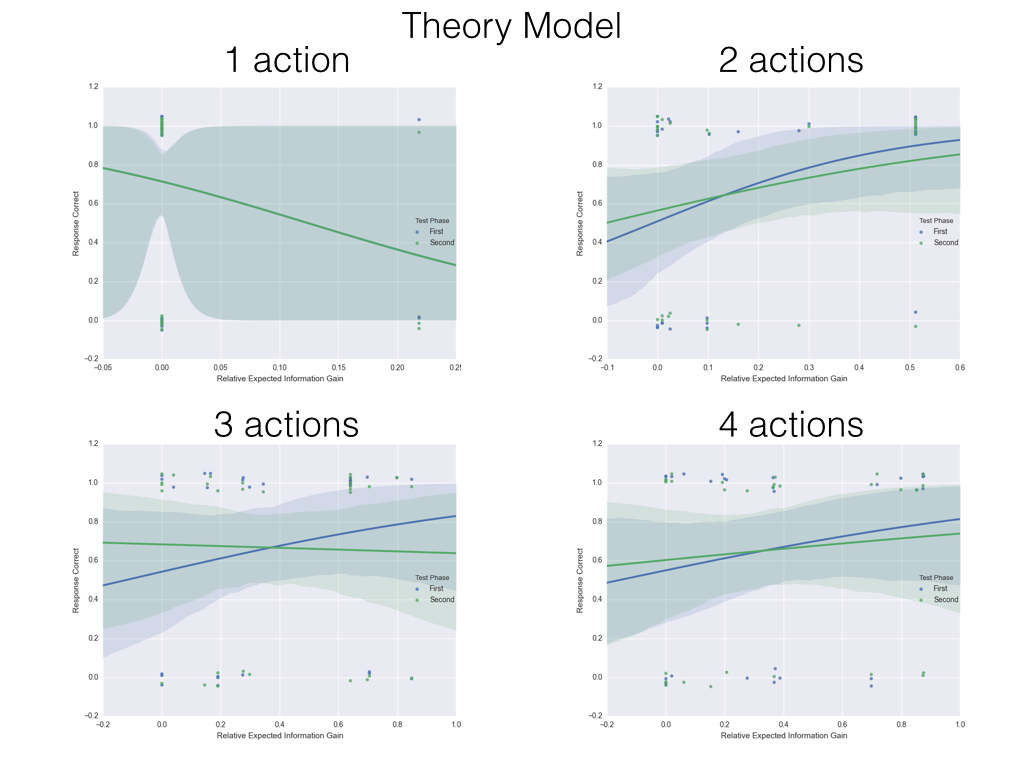
\includegraphics[width=0.75\textwidth]{../Plots/LogRegPlots/LogRegPlots_theory.png}
\end{center}
\caption{Correctness of response in phases 2a (blue) and 2b (green) as a function of EIG relative to theory model in the active learning phase, for the four first actions in this phase.}
\label{fig:logreg_theory}
\end{figure}

\begin{figure}[h!]
\begin{center}
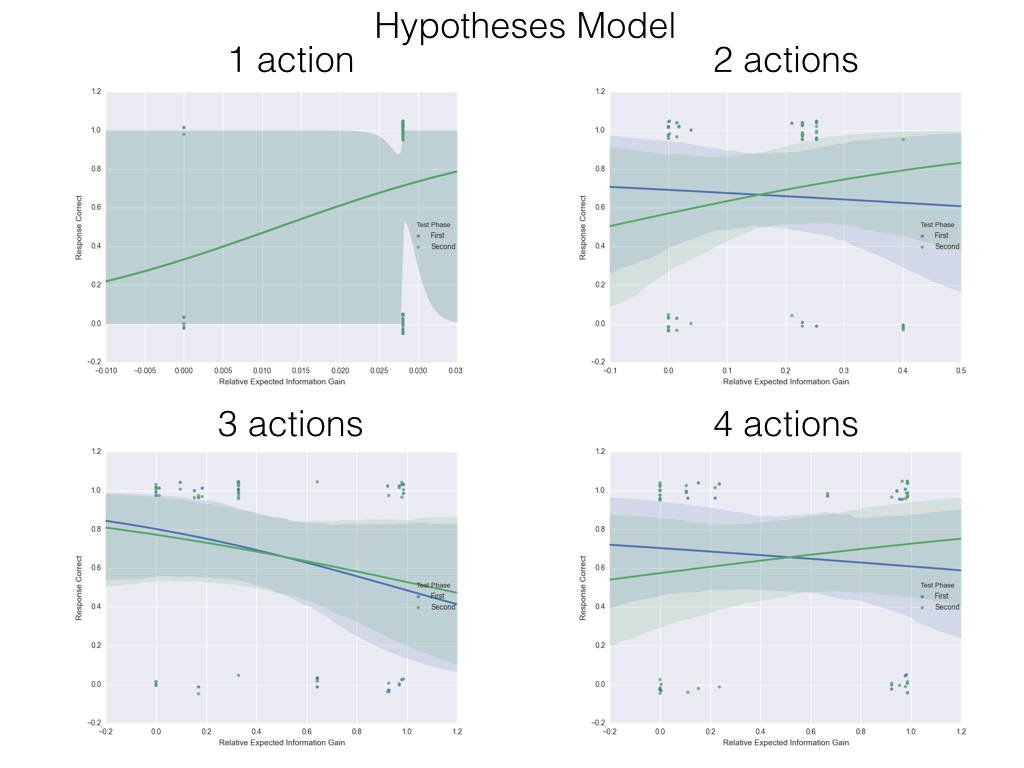
\includegraphics[width=0.75\textwidth]{../Plots/LogRegPlots/LogRegPlots_hypotheses.png}
\end{center}
\caption{Correctness of response in phases 2a (blue) and 2b (green) as a function of EIG relative to hypotheses model in the active learning phase, for the four first actions in this phase.}
\label{fig:logreg_hypotheses}
\end{figure}

\begin{figure}[h!]
\begin{center}
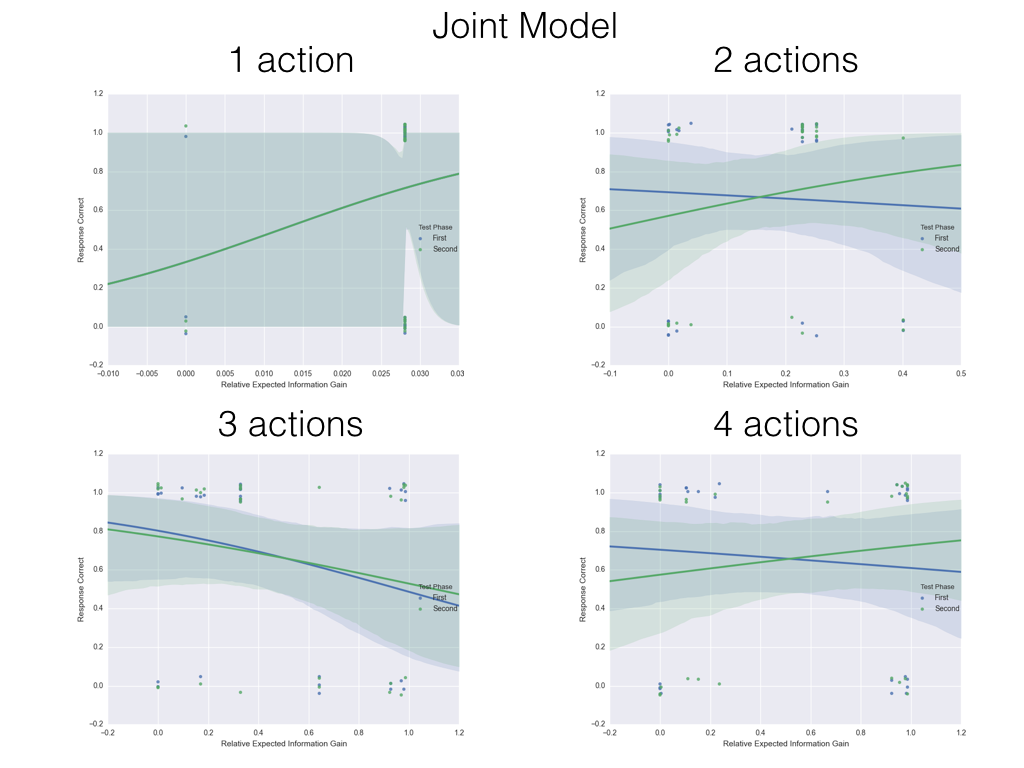
\includegraphics[width=0.75\textwidth]{../Plots/LogRegPlots/LogRegPlots_joint.png}
\end{center}
\caption{Correctness of response in phases 2a (blue) and 2b (green) as a function of EIG relative to joint model in the active learning phase, for the four first actions in this phase. y values (0: incorrect, 1: correct) are jittered for clarity.}
\label{fig:logreg_joint}
\end{figure}

As before, the relative EIG is close to 0 when the kids are performing close to the corresponding optimal model. A positive effect of the active learning phase in the test phase would be seen in these graphs as a decreasing relation, that is, more correct responses for smaller values of EIG. The tendency in the majority of the cases is however the opposite: performance shows a slight increase with increasing relative EIG. These figures are for $\epsilon=0.001$, a value of $\epsilon=0.25$, at the other extreme of the range explored, gives similar results.


\subsection*{Predictive posterior}
The results in the second phase can also be analyzed in terms of the models' predictions, taking into account the experience gathered in the active learning phase. Here, we take the models' choices as those that maximize the probability of activation among the options available to children. Apart from a couple of isolated cases, the experience of the active learning phase allows the models to make perfect predictions in the second phase, so that a direct comparison with children is moot. For phase 2b, the huge dimensionality of the model makes it impossible to run in practice.


\section*{Success Probability}
We now go back to the first phase of the experiment, and consider it in terms of children not maximizing an information gain but instead maximizing the probability of machine activation. We keep filtering identical consecutive actions, which are the maximizing choice, both in the data and in the models, which amounts to including some amount of exploration in the kids' gameplay.

The probability of machine activation (success) for a specific action is given by equation~\eqref{paction}, and is the same for all models. In fact, these probabilities are fixed for the available set of actions, given the prior experience. In order to compare kids performance with a random choice, we define:

\begin{equation}
\mathcal{L_K}=-\log\left(\frac{p^{+}_K}{p^{+}_M}\right)
\end{equation}
for the kids and
\begin{equation}
\mathcal{L_R}=-\log\left(\frac{p^{+}_R}{p^{+}_M}\right)
\end{equation}
for the random choice, where $p^{+}$ are the probabilities of success for the action chosen for the kids ($K$), model ($M$) and random ($R$). 

In figure~\ref{fig:log_pactivation} we show the distribution of these variables for the first four actions ($\epsilon=0.001$). As before, children are plotted in red ($\mathcal{L_K}$) and the random model in blue ($\mathcal{L_R}$). A value close to 0 indicates play consistent with activation probability maximization. 
 
\begin{figure}[h!]
\begin{center}
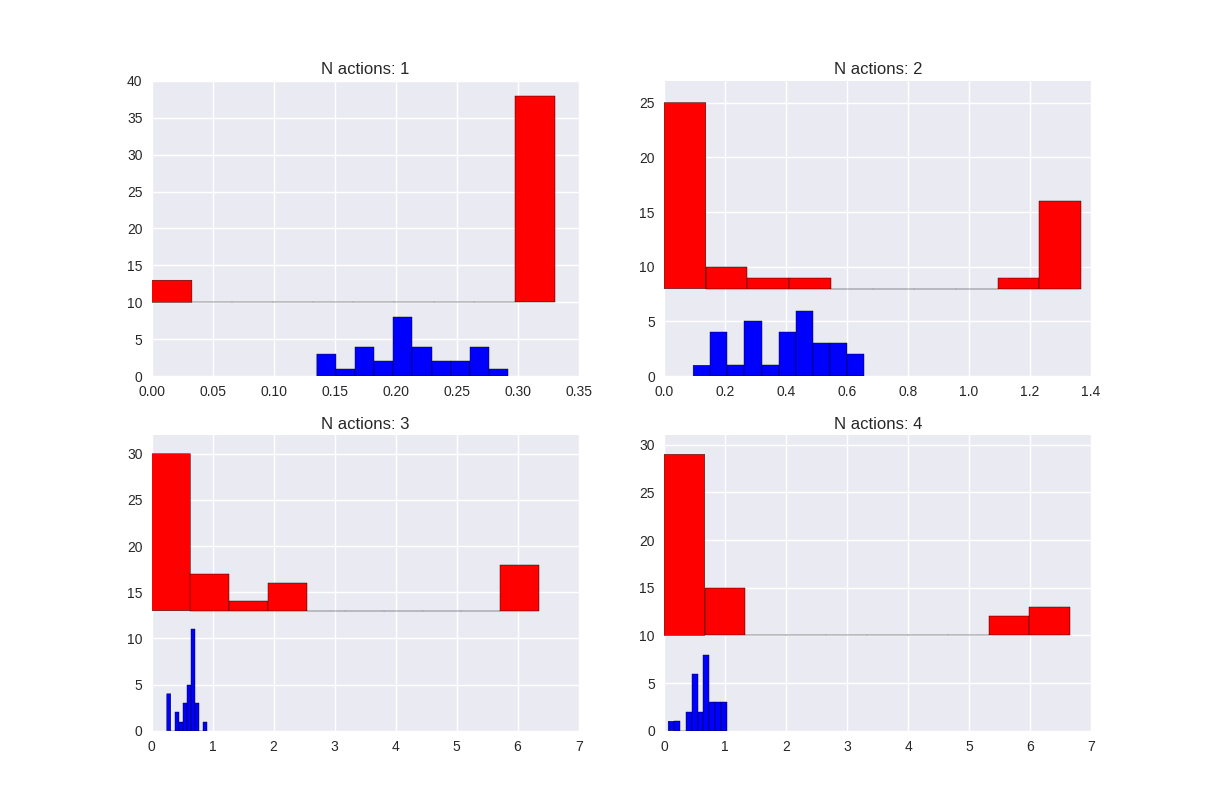
\includegraphics[width=0.75\textwidth]{../Plots/log_pactivation.png}
\end{center}
\caption{Distributions of $\mathcal{L_K}$ (red) and $\mathcal{L_R}$ (blue).}
\label{fig:log_pactivation}
\end{figure}

In mean value, children are consistently worse than random for this measure too. We can try to get rid of the effect of high values by considering the fraction of kids that are better than random for each action number, and test this against chance with a binomial of proportion equal to 1/2. The results are as follows:
\begin{center}
\begin{tabular}{|c||c|c|c|}
\hline
action & $n_{better}$ & $n_{total}$ & p\\
\hline\hline
1 & 3 & 31 & $<10^{-5}$ \\ 
2 & 19 & 30 & 0.200 \\ 
3 & 15 & 30 & 1 \\ 
4 & 19 & 29 & 0.136 \\ 
\hline
\end{tabular}
\end{center}
where $n_{better}$ is the number of kids that are better than random and $n_{total}$ is the total number of kids for that action number (which decreases because some kids performed a smaller amount of actions). We see that for the second and fourth actions a non-significant majority of kids are better than random, and it is tied for the third. In the first actions most kids perform worse than random, but this is likely an artifact of the model's priors. 

Finally, we can try to interpret the apparent bimodality of the plots in figure~\ref{fig:log_pactivation} as a division in a ``player'' population which tries to maximize the probability of activation, and a ``learner'' population which tries to maximize the information gain. The problem with this is that these populations do not seem to be consistent for the different actions. The set of children that perform in a range of $10\%$ of the worst $\mathcal L$ score in the second action (8 kids) has no overlap with that in the third (5 kids). In the fourth action (3 kids) 2 of the kids in the second action reappear, but none of those in the third. 


\end{document}
%    0.25
%    0 & 6.111 & 6.685 & 6.633 \ 
%    1 & 6.145 & 6.611 & 6.625 \ 
%    2 & 6.139 & 6.611 & 6.633 \ 
%    3 & 6.101 & 6.613 & 0.000 \ 
%    4 & 6.105 & 6.610 & 0.000 \ 
%    5 & 6.105 & 6.610 & 6.624 \ 










